

\section{RESULTS}
\subsection{Density projection upon one dimension} % (fold)
\label{ssub:density_projection_upon_one_dimension}


Using Hit-and-Run to sample feasible activation sets, Figure \ref{fig:raw_histograms} shows the distributions of activation solutions for a palmar submaximal force resulting from [briantodo number] solutions computed with Hit-and-Run sampling. This is the first time (to our knowledge) that the internal structure of the feasible activation set has been visualized for a sub-maximal force.
Notice also that the lower and upper bounds of the activations (i.e., the dashed lines that indicate their bounding box), are uniquely uninformative of the actual density of distribution of feasible activations. Note also that the activation needed for the maximal force output (thick gray line) is very often not the mode of the activations at [briantodo select correct number]50\%[maytodo: can we set this as a variable and use throughout?] of output.
\\

Talk about the function of each muscle, with respect to the moment arm matrix and the relevant cell of the A matrix.

The density integrals perpendicular to each muscle are provably unimodal due to the convexity [maytodo cite or add supporting evidence], and therefore it would be inadvisable to fit a normal distribution as the probability density function.
% subsubsection density_projection_upon_one_dimension (end)

\subsection{Activation spaces for increasing force} % (fold)
\label{sub:activation_spaces_for_increasing_force}
For maximal force into any direction, there is a unique activation vector satisfiying all constraint. The maximal force into palmar direction is given by ????? and its unique activation vector ????. [briantodo insert values]
In Figure \ref{fig:Z_progression} we give the distributions of the activations for increasing force, starting with $10\%$ of the maximal force, increasing in $10\%$ steps until maximal force is reached.

\begin{figure}[htbp]
\centering
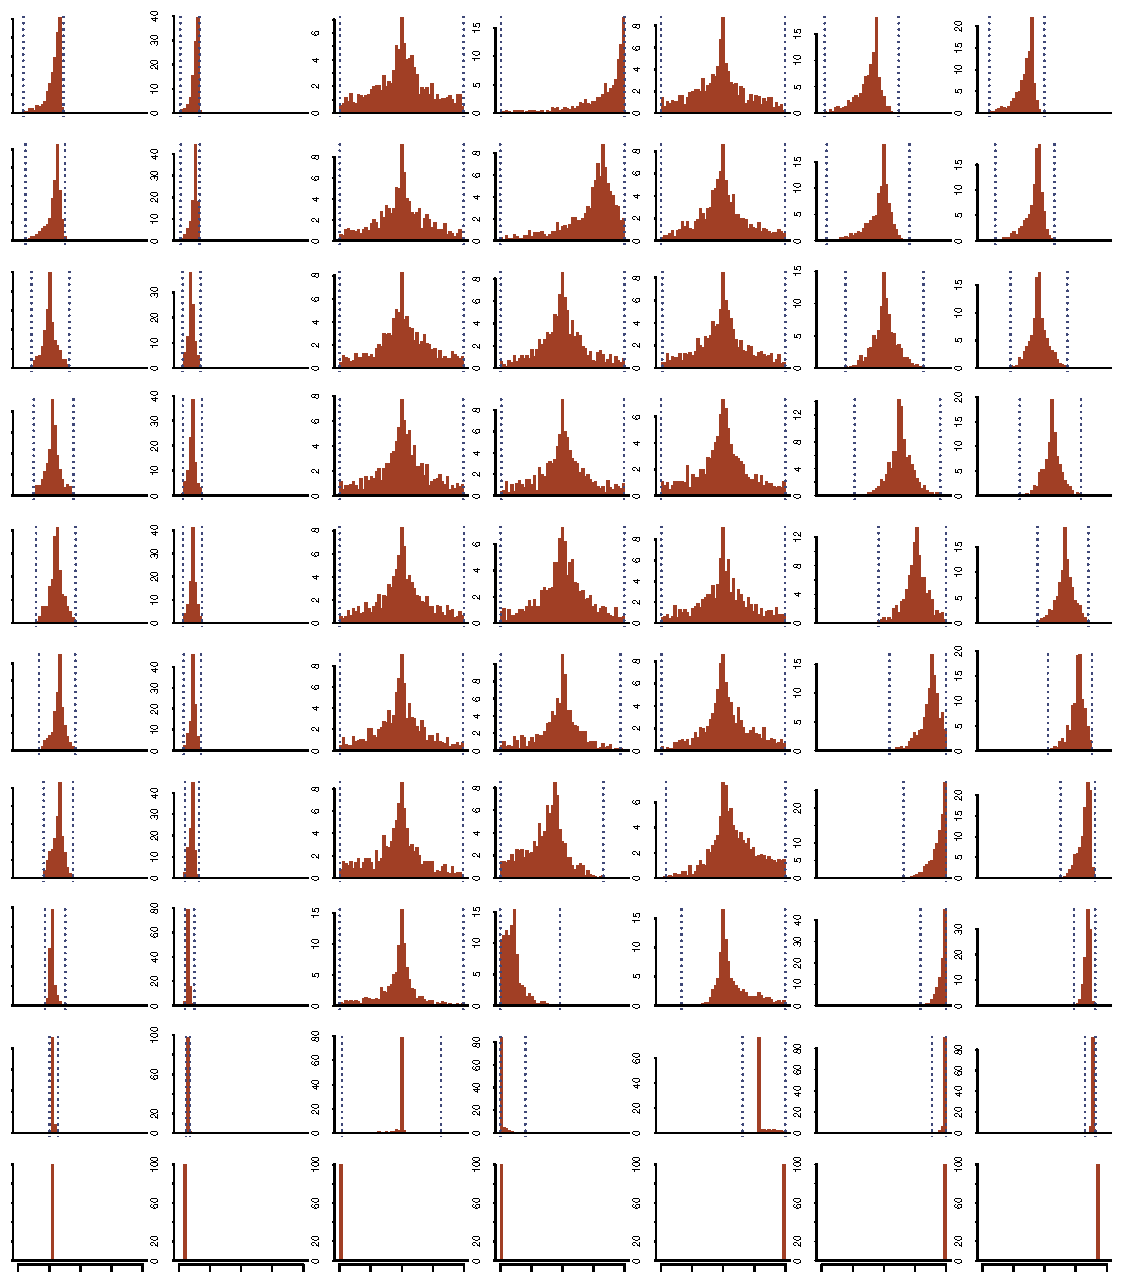
\includegraphics[width=\textwidth]{figs/Z_alphaProgression1430924065026.pdf}
\caption{Distribution of activations in the palmar direction and changing force. Each row of histograms uses a Hit-and-Run set. The height of each bar visualizes the percentage of 10,000 solutions found within a given 0.02 span of activation; the shape is more meaningful than the magnitude of the $y$-axis, as we expect convergence (and therefore peak increase within few bins) towards maximal contractions. We computed the upper and lower bounds of activation for each muscle (vertical dotted lines).}
\label{fig:Z_progression}
\end{figure}% subsection activation_spaces_for_increasing_force (end)

The solution polytope converges as the difficulty of the task increases; the rate of convergence is different across muscles. Whereas for example fds already has a small range of feasible activations at 10\%, EIP has feasible activation $[0,1]$ up to 80\%. For some muscles (such as X and Y) the convergence only occurs in the last [briantodo insert maximal feasible palmar force * 0.90], while others converge earlier-in lower forces of maximal (X and Y are examples of this)[briantodo fill out these descriptive statistics].

It is imperative to keep in mind that every histogram (regardless of its convergence) is composed of the distribution of all 10,000 points; when the distribution is compressed, the relative percentage of the bars will increase, as we fixed break width ($\Delta x$) remain constant to 2\% of maximal contraction. [briantodo cite http://library.msri.org/books/Book31/files/ball.pdf]

The peaks seen in these figures is the perpendicular slice that has the largest relative area; within the same muscle it does not have to be symmetric between the bounds, and can shift over differing tasks.
As expected, the unique solution at 100\% activation appears as a single peak representing 100\% of the sampled points; the bounds and the muscle's unique activation are superimposed.
We explain why these distributions must be unimodal, non-normal, more formally in the discussion, along with information about the structure of the probability density function across a given muscle dimension.
Consider the activation distributions between $\alpha = 0.7$ and $\alpha = 0.8$ for LUM, where the median changed by less than 4\% while the lower bound increased by nearly 13\%.

First, we observe that a meaningful cross-muscle comparison of point distributions cannot be ascertained by the bounding box. For example, at a task of 10\% of maximal palmar force production, EIP and EDC both have lower and upper bounds of 0, and 1, respectively, yet their distributions are thoroughly distinct; the shape of EIP is more symmetric (lower 25\% = 0.36, median = 0.5029, upper 75\% = 0.62), while 75\% of the solutions sampled have edc higher than 0.74 \ref{fig:Z_progression}.

Second, we find this holds not only for inter-muscle distribution comparisons, but intra-muscular distributions. Consider the significant change in the shape of the distributions across the progression for edc until the 60\% task; the lower and upper bounds change less than 1\% and 4\%, respectively, while the median shifted by nearly 40\%.
In the most extreme case, the median activation can be exceptionally narrow, while the bounds are wide- for example, EIP at a 90\% task; although activation is bounded between 0.1 and 0.81, approximately 79\% of the solutions exist with EIP activation between just 0.49 and 0.51.

Next, we see that if one muscle had to be fixed throughout the entire force progression, DI and PI would fail; their bounding boxes of tasks below $\alpha=0.4$ do not include the unique solution at $\alpha=1.0$. We also placed a vertical grey line for the scaled unique solution at maximal, denoted $\textbf{a}^*$, (e.g. LUM converges to an activation of 1 at maximal palmar force, so we put a grey line at 0.8 for $\alpha=0.8$ of maximal palmar force.) Since $\alpha f_{\max} = \alpha A \textbf{a}^*$, $\alpha \textbf{a}^*$ is a solution of the feasible activation set at $\alpha$-fraction of the maximal force. However we observe that for some muscles, these points can lie arbirtraliy in the distribution i.e.\ do not have to lie close to the corresponding peaks (e.g.\ musle DI and EIP).

\subsection{Parallel Coordinates Visualisation}
To maintain realtime interactivity of the plot, we used only the first 1000 points collected for each task, from $\alpha = 0.1$ to $\alpha = 1.0\%$ (maximal force).

\begin{figure}[htbp]
\centering
\includegraphics[width=\textwidth]{figs/parcoord_alpha50.pdf}
\caption{This figure is a snapshot of the interactive platform for visualizing all solutions. This parallel coordinates plot visualizes, where each feasible activation set is strewn across each dimension's axis as a line. While $\alpha$ could be set to view all tasks, we set $\alpha$ to a palmar force of 50\% of the computed maximal feasible force in this direction. Here we show 1000 points accrued from Hit-and-Run on a task of $\alpha=0.5$.}
\label{fig:parcoord_full}
\end{figure}

On the histograms you can predict how many solutions would be lost if you put one constraint on one muscle. Parallel coordinates allow us to visualize not only the amount of solutions lost, but the location of the remaining solutions across the other muscle dimensions. Furthermore one can constraint any number of muscles and still visualize the remaining amount of solutions, whearas in the histogramms one can not make any predictions.

Figure \ref{fig:parcoord_full} is a modified screen-shot of the platform, constrain activation for a given muscle or cost function from above, below, or both. The resulting number of lines represents how the solution space changed across all dimensions recorded.
Note how $\alpha$ can also be constrained- we can explore one or more levels of force output at a time.

\begin{figure}[htbp]
\centering
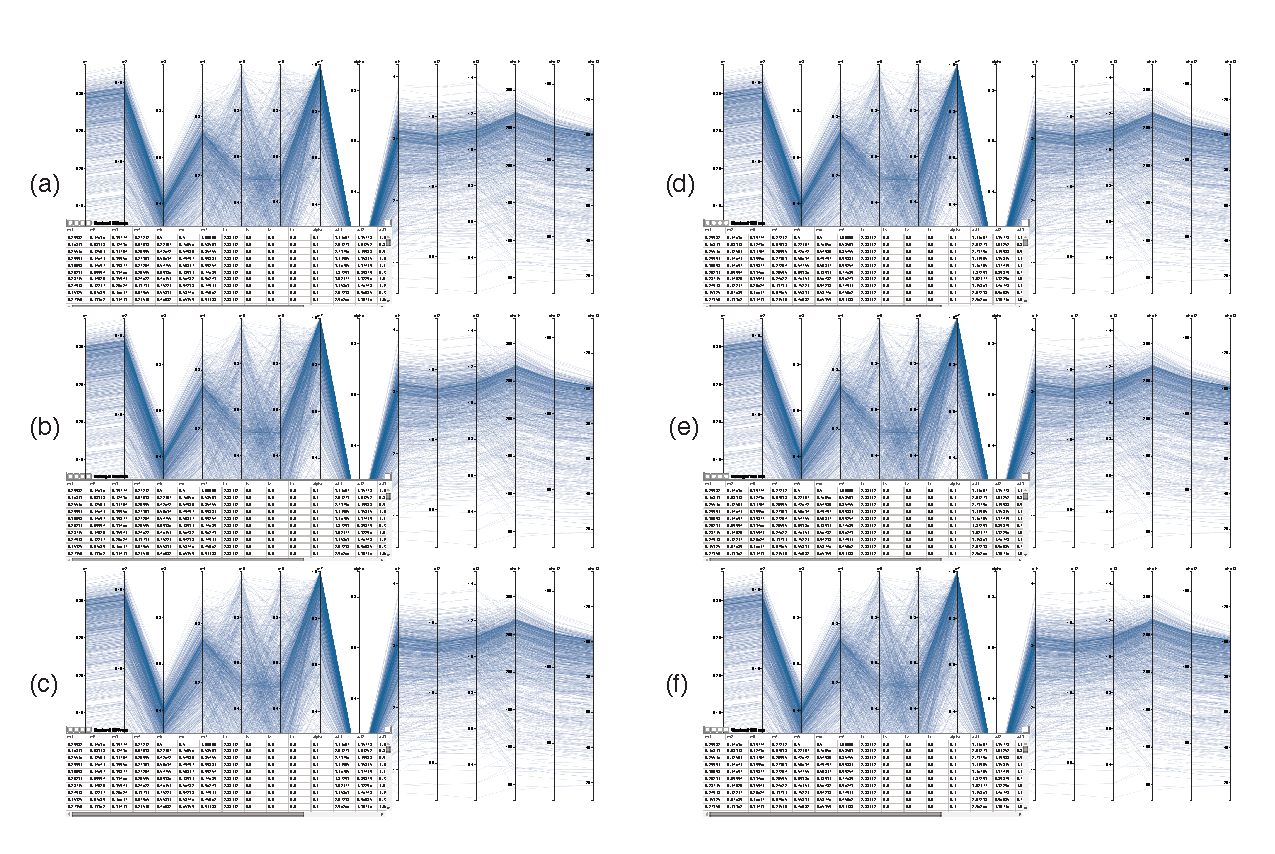
\includegraphics[width=\textwidth]{figs/parcoords.pdf}
\caption{These snapshots show the use of the interactive parallel coordinate visualization of solutions across the activation space. For the task set to 50\% of maximal in the palmar direction, we show the
(a) remaining 166 solutions when PI $<$ 60\% 
(b) remaining 57 solutions when DI $<$ 60\%, and the
(c) remaining 57 solutions when we constrain PI $<$ 60\% and DI $<$ 60\%. We also show the
(d) remaining 502 solutions when we select the lower 50\% of $l_1$ costs,
(e) remaining 498 solutions when we select the lower 50\% of $l_2^w$ costs, and the
(f) remaining 220 solutions when we select the lower 50\% across all cost functions in Table \ref{cost_function_tabls} }
\label{fig:parcoords}
\end{figure}

Constraining PI $<$ 60\% still leaves a solution space about three times as large as di $<$ 60\%. 
Observe that constraining di $<$ 60\% already implies that PI $<$ 60\% as seen in Figure \ref{fig:parcoords} (b), (c). 
Constraining one muscles does have different effects on the other muscles as for example if ei is constrained below 60\% activation, we see that the bounding box of PI is significantly restricted; however, the same constraint has no effect on the bounding box of EIP.

discuss what happens when you bring each of those muscles down, using the R produced stats.
talk about how when you add X as a constraint, most of the solutions are distributed across the other muscles between X and X. Say which ones go up, which go down- which ones become clustered and which ones lose their peak/spike.

As there are only few not steep crossings between $l_1$, $l_2$ and $l_3$, the parallel coordintes suggest correlation of those three weights. Similar correlation is observerved for the respective weighted functions. %the unweighted l1,l2,and l3 cost functions for the finger were highly correlated with one another, and the weighted functions were similarly correlated, 
We provide a scatter plot for their relationships in Appendix Figures \ref{fig:unweighted_cost_functions} and \ref{fig:weighted_cost_functions}.

% subsection parallel_coordinates (end)